%% ============================================================
%% MALTG-DSR — Artículo científico formato MDPI (revista Computers)
%% Compilar: pdflatex paper && bibtex paper && pdflatex paper && pdflatex paper
%% ============================================================
\documentclass[computers,article,submit,pdftex,moreauthors]{Definitions/mdpi}

%% Paquetes para figuras y matemáticas
\usepackage{tikz}
\usetikzlibrary{arrows.meta,positioning,shapes.geometric,fit,backgrounds,calc}
\usepackage{pgfplots}
\pgfplotsset{compat=1.17}

%% Castellanización de etiquetas de flotantes
\renewcommand{\figurename}{Figura}
\renewcommand{\tablename}{Tabla}

%% Metadatos del número (placeholder de envío)
\firstpage{1}
\makeatletter
\setcounter{page}{\@firstpage}
\makeatother
\pubvolume{15}
\issuenum{1}
\articlenumber{0}
\pubyear{2026}
\copyrightyear{2026}
\datereceived{ }
\daterevised{ }
\dateaccepted{ }
\datepublished{ }

%% ── Título ─────────────────────────────────────────────────
\Title{Ciencia del Diseño para la Gobernanza Digital Judicial: MALTG como Teoría de Diseño Naciente --- Sombras Digitales Semánticas, Razonamiento Normativo Anti-Alucinación y Ciclo Adaptativo MAPE-K Evaluados con Instrumentos de Validez en el Ecosistema de Justicia del Ecuador}

%% ── Autoría (reemplazar con datos definitivos) ─────────────
\newcommand{\orcidauthorA}{0000-0000-0000-0000}
\Author{Patricio Michael~Autor $^{1,}$*}
\AuthorNames{Patricio Michael Autor}
\address{$^{1}$ \quad Programa de Doctorado / Facultad de Ingeniería; correo institucional}
\corres{Correspondencia: pat\_mic@hotmail.com}

%% ── Resumen ────────────────────────────────────────────────
\abstract{La gobernanza de los ecosistemas digitales judiciales carece de artefactos que sean simultáneamente automatizados, semánticamente fundados, verificables y adaptativos. Este artículo aplica el paradigma de investigación en ciencia del diseño (Design Science Research, DSR) para construir y evaluar MALTG, una suite integrada de artefactos para la gobernanza digital LegalTech instanciada como plataforma contenedorizada y evaluada en el ecosistema de justicia del Ecuador. Siguiendo la metodología DSRM y los tres ciclos de relevancia, rigor y diseño, la suite articula: (i) \emph{constructos} ---cobertura jerárquica $\Psi$, brecha $\delta$, salud procesal, variabilidad fáctica y deriva de proceso---; (ii) \emph{modelos} ---ontología de gobernanza multiestándar de 131 conceptos, ontología ejecutable del COGEP y sombras digitales JSON-LD---; (iii) \emph{métodos} ---ingesta no invasiva de evidencia web, razonador normativo determinista con barrera anti-alucinación, notarización por cadena de hashes y ciclo adaptativo MAPE-K---; y (iv) una \emph{instanciación} operativa con 40 endpoints. La evaluación, organizada con el marco FEDS en cinco episodios formativos y sumativos, combina verificación estructural de la ontología (10 preguntas de competencia satisfechas), un escenario artificial de cobertura ($\Psi_{\mathrm{global}} = 0{,}905$), un despliegue naturalista sobre 47 causas reales (60 términos evaluados, puntualidad 36{,}7\%), análisis de sensibilidad ($\Psi_{\mathrm{global}} \in [0{,}9035,\, 0{,}9053]$ ante perturbaciones de $\pm 20\%$ con ordenamiento de brechas invariante) e instrumentos de validez experta (kappa de Cohen, CVR de Lawshe, consistencia AHP, concordancia de Spearman). Como escenario pragmático, se documenta el recorrido completo de auditoría del Consejo de la Judicatura. La contribución se posiciona como mejora en el cuadrante de Gregor--Hevner y se destila en seis principios de diseño transferibles que configuran una teoría de diseño naciente para la gobernanza digital de ecosistemas judiciales.}

%% ── Palabras clave ─────────────────────────────────────────
\keyword{ciencia del diseño; DSR; gobernanza digital; LegalTech; ontologías; sombra digital; MAPE-K; validación experta; justicia electrónica; teoría de diseño}

\begin{document}

%% ============================================================
\section{Introducción}
\label{sec:intro}

Los sistemas judiciales digitalizados plantean un problema de gobernanza doblemente difícil. Por un lado, sus ecosistemas tecnológicos ---portales, sistemas de gestión procesal, repositorios estadísticos--- son heterogéneos, opacos y difíciles de auditar de forma continua \cite{Rosa2013,Lupo2014}; por otro, la incorporación de inteligencia artificial agrava el riesgo, pues los modelos generativos alucinan contenido jurídico con tasas del 58--82\% \cite{Dahl2024}, que las herramientas comerciales con recuperación aumentada solo reducen al 17--33\% \cite{Magesh2025}, un nivel inaceptable cuando las salidas inciden en derechos procesales \cite{Rudin2019}. La literatura ofrece piezas sueltas ---gemelos y sombras digitales \cite{Kritzinger2018,Jones2020,Brauner2022}, ontologías jurídicas \cite{BenchCapon2012,Casanovas2016}, integración neuro-simbólica \cite{Sarker2021,Pan2024}, libros mayores gubernamentales \cite{Olnes2017}, datos abiertos \cite{Janssen2012,Attard2015}---, pero no un artefacto integrado, evaluado y teóricamente destilado que las articule para el dominio judicial. La revisión de Karabulut et al.\ identifica además que la validación de la correspondencia entre modelos semánticos y sistemas representados es un problema abierto de los gemelos digitales \cite{Karabulut2024}.

Este vacío es, en esencia, un problema de \emph{diseño}: no se trata de explicar un fenómeno existente sino de crear y evaluar artefactos útiles que lo resuelvan. Por ello adoptamos el paradigma de investigación en ciencia del diseño (DSR) \cite{Hevner2004,March1995}, ejecutado conforme a la metodología DSRM de Peffers et al.\ \cite{Peffers2007}, evaluado con el marco FEDS \cite{Venable2016} y comunicado según el esquema de contribución de Gregor y Hevner \cite{Gregor2013}, buscando el equilibrio entre artefacto y teoría que reclama la comunidad \cite{Baskerville2018,GregorJones2007}.

El resultado es MALTG (\emph{Multidimensional Adaptive LegalTech Governance}), una suite de artefactos instanciada como plataforma contenedorizada y evaluada con datos reales del ecosistema de justicia del Ecuador. Las contribuciones son: (1) la \textbf{suite de artefactos} completa ---constructos, modelos, métodos e instanciación en la taxonomía de March y Smith \cite{March1995}--- para la gobernanza digital judicial; (2) un \textbf{escenario pragmático} documentado de extremo a extremo que demuestra el artefacto sobre el Consejo de la Judicatura y 47 causas reales; (3) una \textbf{evaluación multi-episodio} conforme a FEDS que combina verificación formal, escenarios artificiales, despliegue naturalista, análisis de sensibilidad e instrumentos de validez experta; y (4) una \textbf{teoría de diseño naciente} ---seis principios transferibles y los ocho componentes de Gregor y Jones \cite{GregorJones2007}--- para artefactos de gobernanza en dominios normativos de alto riesgo.

%% ============================================================
\section{Metodología: Ciencia del Diseño}
\label{sec:dsr}

La investigación se organizó según los tres ciclos de Hevner \cite{Hevner2004}: el \emph{ciclo de relevancia} conecta con el entorno del problema (la judicatura ecuatoriana, sus expedientes públicos, el COGEP y las partes procesales); el \emph{ciclo de rigor} ancla el diseño en la base de conocimiento (gemelos digitales, ingeniería ontológica \cite{Gruber1993,Uschold1996,Guarino2002}, verificación de conformidad \cite{Rozinat2008}, criptografía de integridad \cite{Haber1991}, computación autonómica \cite{Kephart2003}); y el \emph{ciclo de diseño} itera construcción y evaluación del artefacto. La Figura~\ref{fig:ciclos} esquematiza la correspondencia y la Tabla~\ref{tab:dsrm} mapea las seis actividades de la DSRM \cite{Peffers2007} a los productos concretos de esta investigación.

\begin{figure}[H]
\centering
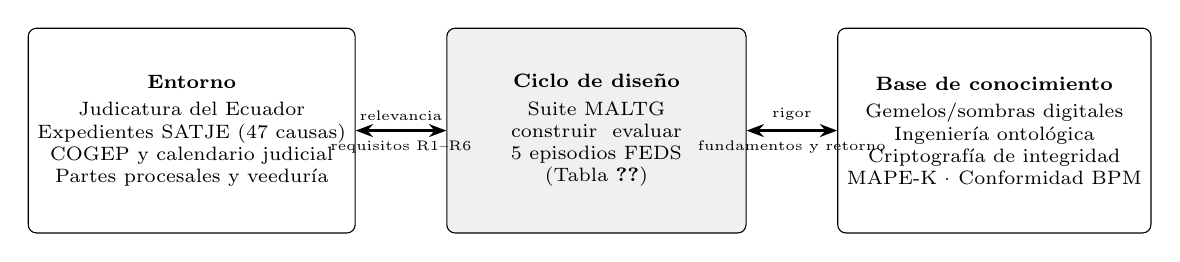
\begin{tikzpicture}[
  box/.style={draw, rounded corners=3pt, align=center, font=\scriptsize, minimum height=2.6cm, minimum width=3.4cm},
  mid/.style={draw, rounded corners=3pt, align=center, font=\scriptsize, minimum height=2.6cm, minimum width=3.8cm, fill=gray!12},
  arr/.style={{Stealth[length=2.2mm]}-{Stealth[length=2.2mm]}, thick}]
\node[box] (env) {\textbf{Entorno}\\[2pt]Judicatura del Ecuador\\Expedientes SATJE (47 causas)\\COGEP y calendario judicial\\Partes procesales y veeduría};
\node[mid, right=1.15cm of env] (des) {\textbf{Ciclo de diseño}\\[2pt]Suite MALTG\\construir $\rightleftarrows$ evaluar\\5 episodios FEDS\\(Tabla \ref{tab:feds})};
\node[box, right=1.15cm of des] (kb) {\textbf{Base de conocimiento}\\[2pt]Gemelos/sombras digitales\\Ingeniería ontológica\\Criptografía de integridad\\MAPE-K · Conformidad BPM};
\draw[arr] (env) -- node[above, font=\tiny]{relevancia} node[below, font=\tiny]{requisitos R1--R6} (des);
\draw[arr] (des) -- node[above, font=\tiny]{rigor} node[below, font=\tiny]{fundamentos y retorno} (kb);
\end{tikzpicture}
\caption{Los tres ciclos de la investigación en ciencia del diseño \cite{Hevner2004} instanciados en MALTG.}
\label{fig:ciclos}
\end{figure}

\begin{table}[H]
\caption{Actividades de la metodología DSRM \cite{Peffers2007} y su materialización en esta investigación.}
\label{tab:dsrm}
\begin{tabularx}{\textwidth}{lXX}
\toprule
\textbf{Actividad DSRM} & \textbf{Materialización} & \textbf{Producto verificable}\\
\midrule
1. Identificación del problema & Gobernanza judicial no auditable; IA jurídica no confiable \cite{Rosa2013,Dahl2024} & Requisitos R1--R6 (Tabla~\ref{tab:reqs})\\
2. Objetivos de la solución & Gobernanza automatizada, fundada, verificable y adaptativa & Objetivos de diseño por requisito\\
3. Diseño y desarrollo & Suite de artefactos MALTG (constructos, modelos, métodos, instanciación) & Plataforma Docker; 40 endpoints REST\\
4. Demostración & Escenario pragmático de extremo a extremo & Sección~\ref{sec:escenario}\\
5. Evaluación & Cinco episodios FEDS \cite{Venable2016} & Sección~\ref{sec:eval}; Tabla~\ref{tab:feds}\\
6. Comunicación & Contribución tipo mejora \cite{Gregor2013}; teoría naciente \cite{GregorJones2007} & Este artículo; Tablas~\ref{tab:dp} y \ref{tab:teoria}\\
\bottomrule
\end{tabularx}
\end{table}

Del ciclo de relevancia se derivaron seis requisitos que todo artefacto de gobernanza digital judicial debe satisfacer, cada uno anclado en deficiencias documentadas por la literatura (Tabla~\ref{tab:reqs}).

\begin{table}[H]
\caption{Requisitos de diseño derivados del ciclo de relevancia y mecanismo que los satisface.}
\label{tab:reqs}
\begin{tabularx}{\textwidth}{lXX}
\toprule
\textbf{Req.} & \textbf{Enunciado (deficiencia que corrige)} & \textbf{Mecanismo en MALTG}\\
\midrule
R1 & Observación automatizada y no invasiva del ecosistema \cite{Rosa2013} & Ingesta de evidencia web con agente identificado y hash de captura\\
R2 & Fundamento semántico compartido \cite{Karabulut2024,Casanovas2016} & Ontologías OWL 2 (gobernanza y COGEP) + sombras JSON-LD\\
R3 & Medición del alineamiento modelo--realidad \cite{Karabulut2024} & Cobertura $\Psi$, brecha $\delta$, conformidad IVF/IDP\\
R4 & Salidas de IA sin alucinación y con procedencia \cite{Dahl2024,Rudin2019} & Razonador determinista + barrera de frontera ontológica\\
R5 & Integridad verificable del expediente \cite{Haber1991,Olnes2017} & Cadena de hashes SHA-256 + bitácora de solo escritura\\
R6 & Adaptación ante cambio normativo y deriva \cite{Kephart2003} & Ciclo MAPE-K con changelog de la KB y análisis de impacto\\
\bottomrule
\end{tabularx}
\end{table}

%% ============================================================
\section{El Artefacto: Suite MALTG}
\label{sec:artefacto}

Conforme a la taxonomía de March y Smith \cite{March1995}, la suite comprende artefactos de los cuatro tipos (Tabla~\ref{tab:tipos}), integrados en la arquitectura de la Figura~\ref{fig:arch}.

\begin{table}[H]
\caption{Inventario de la suite MALTG según la taxonomía de artefactos de ciencia del diseño \cite{March1995}.}
\label{tab:tipos}
\begin{tabularx}{\textwidth}{lX}
\toprule
\textbf{Tipo} & \textbf{Artefactos}\\
\midrule
Constructos & Cobertura jerárquica $\Psi$; brecha de gobernanza $\delta$; salud procesal $S$; índice de variabilidad fáctica IVF; índice de deriva procesal IDP; riesgo $\rho$; tasa de alucinación emitida $\mathcal{H}$; niveles de madurez $L$.\\
Modelos & Ontología de gobernanza multiestándar $\Omega$ (131 conceptos, 144 relaciones; TOGAF, COBIT, ITIL, NIST CSF, IA, cadena de bloques, datos abiertos, seguridad, interoperabilidad, dominio LegalTech); ontología ejecutable del COGEP $\Omega_L$ (7 procedimientos, 16 actos, 11 reglas, 55 feriados); sombras digitales estructurales JSON-LD; gemelo de flujo BPMN (171 actividades, 79 flujos).\\
Métodos & Protocolo de ingesta web no invasiva; motor de validación $\Psi/\delta$; razonador normativo con barrera anti-alucinación; notarización por cadena de hashes; proyección a datos abiertos JSON-LD/DCAT; ciclo adaptativo MAPE-K (M1--M6); instrumentos de validez experta (A1--A5).\\
Instanciación & Plataforma contenedorizada (Docker) con backend FastAPI ($\sim$3500 líneas, 40 endpoints REST) y frontend de visualización interactiva (13 vistas: metodología, ontologías, sombra, validación, workflow, razonador, bitácora, ciclo adaptativo, validación experta).\\
\bottomrule
\end{tabularx}
\end{table}

\begin{figure}[H]
\centering
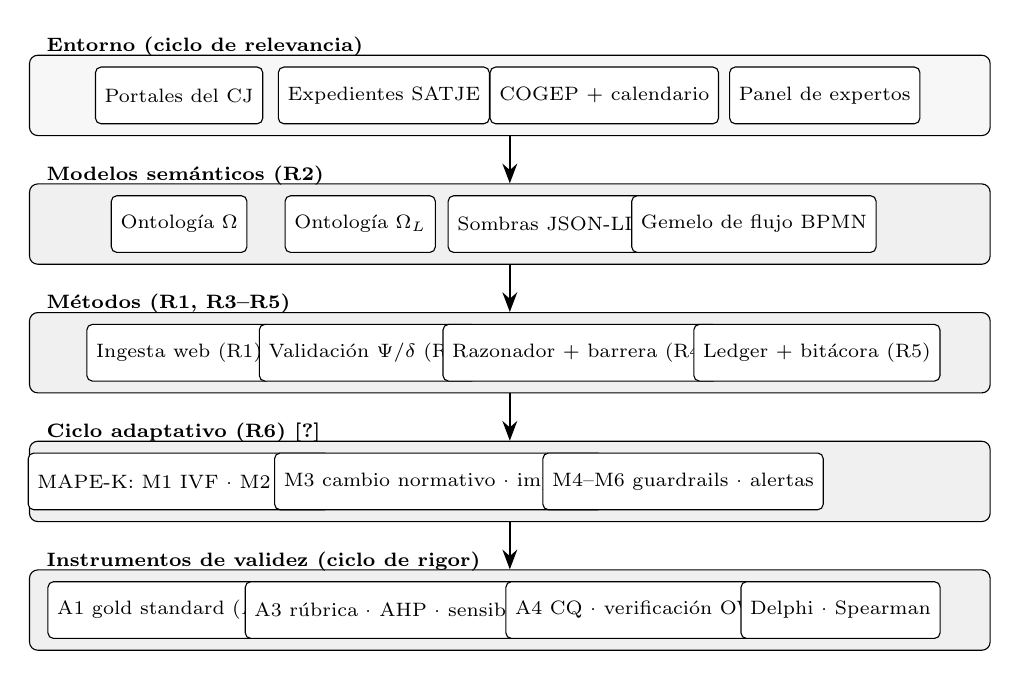
\begin{tikzpicture}[
  capa/.style={draw, rounded corners=3pt, minimum width=12.2cm, minimum height=1.02cm, align=center, font=\small},
  comp/.style={draw, rounded corners=2pt, minimum height=0.72cm, align=center, font=\scriptsize, fill=white},
  flow/.style={-{Stealth[length=2.5mm]}, thick}]
\node[capa, fill=gray!6]  (l1) {};
\node[comp] at ($(l1.center)+(-4.2,0)$) {Portales del CJ};
\node[comp] at ($(l1.center)+(-1.6,0)$) {Expedientes SATJE};
\node[comp] at ($(l1.center)+(1.2,0)$)  {COGEP + calendario};
\node[comp] at ($(l1.center)+(4.0,0)$)  {Panel de expertos};
\node[font=\scriptsize\bfseries, anchor=west] at ($(l1.west)+(0.1,0.62)$) {Entorno (ciclo de relevancia)};

\node[capa, below=0.6cm of l1, fill=gray!12] (l2) {};
\node[comp] at ($(l2.center)+(-4.2,0)$) {Ontología $\Omega$};
\node[comp] at ($(l2.center)+(-1.9,0)$) {Ontología $\Omega_L$};
\node[comp] at ($(l2.center)+(0.5,0)$)  {Sombras JSON-LD};
\node[comp] at ($(l2.center)+(3.1,0)$)  {Gemelo de flujo BPMN};
\node[font=\scriptsize\bfseries, anchor=west] at ($(l2.west)+(0.1,0.62)$) {Modelos semánticos (R2)};

\node[capa, below=0.6cm of l2, fill=gray!12] (l3) {};
\node[comp] at ($(l3.center)+(-4.2,0)$) {Ingesta web (R1)};
\node[comp] at ($(l3.center)+(-1.8,0)$) {Validación $\Psi/\delta$ (R3)};
\node[comp] at ($(l3.center)+(0.9,0)$)  {Razonador + barrera (R4)};
\node[comp] at ($(l3.center)+(3.9,0)$)  {Ledger + bitácora (R5)};
\node[font=\scriptsize\bfseries, anchor=west] at ($(l3.west)+(0.1,0.62)$) {Métodos (R1, R3--R5)};

\node[capa, below=0.6cm of l3, fill=gray!12] (l4) {};
\node[comp] at ($(l4.center)+(-4.2,0)$) {MAPE-K: M1 IVF · M2 drift};
\node[comp] at ($(l4.center)+(-0.9,0)$) {M3 cambio normativo · impacto};
\node[comp] at ($(l4.center)+(2.2,0)$)  {M4--M6 guardrails · alertas};
\node[font=\scriptsize\bfseries, anchor=west] at ($(l4.west)+(0.1,0.62)$) {Ciclo adaptativo (R6) \cite{Kephart2003}};

\node[capa, below=0.6cm of l4, fill=gray!12] (l5) {};
\node[comp] at ($(l5.center)+(-4.2,0)$) {A1 gold standard ($F_1$, $\kappa$)};
\node[comp] at ($(l5.center)+(-1.3,0)$) {A3 rúbrica · AHP · sensibilidad};
\node[comp] at ($(l5.center)+(1.7,0)$)  {A4 CQ · verificación OWL};
\node[comp] at ($(l5.center)+(4.2,0)$)  {Delphi · Spearman};
\node[font=\scriptsize\bfseries, anchor=west] at ($(l5.west)+(0.1,0.62)$) {Instrumentos de validez (ciclo de rigor)};

\draw[flow] (l1) -- (l2);
\draw[flow] (l2) -- (l3);
\draw[flow] (l3) -- (l4);
\draw[flow] (l4) -- (l5);
\end{tikzpicture}
\caption{Arquitectura de la instanciación MALTG: cada capa materializa requisitos del ciclo de relevancia con fundamentos del ciclo de rigor.}
\label{fig:arch}
\end{figure}

\subsection{Núcleo Formal}
El núcleo matemático de la suite se resume en cinco familias de definiciones. Primero, la validación del alineamiento modelo--realidad (R3) se funda en la quíntupla $\mathcal{M} = \langle \Omega, \Delta, \Gamma, \Psi, \delta \rangle$, donde $\Gamma: V \rightarrow 2^{C}$ ancla los componentes de la sombra digital $\Delta = G(V,E,\lambda)$ a los conceptos de $\Omega$, induciendo el conjunto de cobertura $R = \bigcup_{v \in V} \Gamma(v)$. Para cada dimensión de gobernanza $d$ con raíz $r_d$ y subconceptos $S_d$:
\begin{equation}
\Psi(d) = w_r \cdot \mathbb{1}[r_d \in R] + w_s \cdot \frac{|S_d \cap R|}{|S_d|},
\qquad
\delta(d) = \mathrm{onto}(d)\bigl(1 - \Psi(d)\bigr),
\label{eq:psi}
\end{equation}
con pesos $(w_r, w_s)$ calibrables por AHP \cite{Saaty1990}. Segundo, el razonamiento normativo (R4) computa veredictos de término en días hábiles $d_H$ sobre el calendario judicial, con función escalonada de tolerancia $\alpha = 1{,}25$ y salud procesal
\begin{equation}
S(c) = \frac{1}{|\mathcal{R}_c|} \sum_{r \in \mathcal{R}_c} \pi\bigl(V(r,c)\bigr),
\qquad
\pi(\textsc{cumple}, \textsc{alerta}, \textsc{incumple}) = (100, 60, 0).
\label{eq:salud}
\end{equation}
Tercero, la conformidad estructural entre la traza real y el flujo canónico \cite{Rozinat2008} se mide con $\mathrm{IVF}(c) = 100\,(|E_c|+|M_c|)/(|K_c|+|E_c|)$ y con el índice de deriva $\mathrm{IDP}(c)$, agregándose en el riesgo $\rho(c) = 0{,}50\,(100-S(c)) + 0{,}25\,\mathrm{IVF}(c) + 0{,}25\,\mathrm{IDP}(c)$. Cuarto, la barrera anti-alucinación (R4) restringe toda salida al cierre $\mathrm{Th}(\Omega_L \cup F_c)$, de modo que la tasa de alucinación emitida es nula por construcción sobre el dominio tipificado y todo lo ajeno al vocabulario ontológico se reporta como \emph{fuera de frontera}, nunca se genera. Quinto, la integridad (R5) encadena las actuaciones con $b_i = h(i \,\|\, t_i \,\|\, h(x_i) \,\|\, b_{i-1})$ \cite{Haber1991}, con evidencia de manipulación demostrable por inducción.

\subsection{Instrumentos de Validez del Ciclo de Rigor}
La suite incorpora como artefactos de primera clase los instrumentos con que se evalúa a sí misma ---una decisión de diseño que convierte el rigor en característica operativa. El módulo A1 permite a juristas anotar un estándar de oro sobre las actuaciones y evalúa el reconocimiento de actos del razonador con precisión, exhaustividad, $F_1$ y el coeficiente kappa de Cohen \cite{Cohen1960}
\begin{equation}
\kappa = \frac{p_o - p_e}{1 - p_e},
\label{eq:kappa}
\end{equation}
que corrige la concordancia observada $p_o$ por la esperada por azar $p_e$. El módulo A3 gestiona la rúbrica de evidencias por dimensión (escala 0--100 en cinco niveles), los juicios AHP sobre los pesos $(w_r, w_s)$ con verificación de consistencia
\begin{equation}
\mathrm{CI} = \frac{\lambda_{\max} - n}{n - 1}, \qquad \mathrm{CR} = \mathrm{CI}/\mathrm{RI} < 0{,}10,
\label{eq:ahp}
\end{equation}
\cite{Saaty1990}, y el análisis de sensibilidad que perturba los pesos $\pm 10\%$ y $\pm 20\%$. El módulo A4 genera la ontología COGEP en OWL 2 desde la base de conocimiento, ejecuta verificación estructural y responde las preguntas de competencia \cite{Uschold1996}; la validez de contenido de conceptos y reglas se cuantifica con la razón de Lawshe $\mathrm{CVR} = (n_e - N/2)/(N/2)$ \cite{Lawshe1975}. Finalmente, la ponderación de dimensiones por panel (método Delphi, escala 1--9) computa la concordancia inter-experto con el coeficiente de Spearman \cite{Spearman1904}
\begin{equation}
r_s = 1 - \frac{6 \sum_i d_i^2}{n(n^2-1)}.
\label{eq:spearman}
\end{equation}
Toda operación de estos instrumentos ---anotación, juicio, evidencia, cambio de supuestos--- se asienta en la bitácora encadenada, de modo que la propia evaluación del artefacto es auditable (R5).

%% ============================================================
\section{Demostración: Escenario Pragmático}
\label{sec:escenario}

Conforme a la actividad 4 de la DSRM \cite{Peffers2007}, se documenta el uso del artefacto en un escenario real de extremo a extremo con cuatro actores del ecosistema de justicia ecuatoriano. La Tabla~\ref{tab:escenario} resume cada paso con su salida verificable real.

\textbf{Paso 1 --- El auditor de gobernanza.} Ejecuta la ingesta no invasiva sobre los portales públicos del Consejo de la Judicatura. El sistema detecta las señales del ecosistema (gestor de contenido genérico, 19 enlaces a aplicaciones heredadas, SPA procesal sin API pública, ausencia de JSON-LD) y genera la sombra digital fechada \texttt{LegalTech\_funcionjudicial} (34 componentes, 32 flujos, 7 capas) con índice de madurez 46/100 ---nivel 3, «Definido»--- y la interoperabilidad semántica como dimensión más débil (28/100). El radar y las brechas quedan disponibles para comparación longitudinal.

\textbf{Paso 2 --- La jueza de unidad civil.} Carga una causa de inquilinato (10 actuaciones, procedimiento sumario). El gemelo de flujo BPMN resalta el recorrido de la causa sobre el flujo canónico; el razonador evalúa 4 términos COGEP y dictamina salud $S = 65/100$ (2 \textsc{cumple}, 1 \textsc{alerta}, 1 \textsc{incumple}), citando para cada veredicto el artículo aplicado, las fechas comparadas y los días hábiles computados. El chat COGEP responde únicamente dentro de la frontera ontológica; la consulta «¿qué plazos se incumplieron?» devuelve la regla, el artículo y el exceso en días, con el hash de la base normativa.

\textbf{Paso 3 --- Las partes procesales y la veeduría.} Verifican en línea la cadena de notarización (10 bloques SHA-256; alterar una actuación rompe la cadena) y descargan el expediente como datos abiertos JSON-LD/DCAT con licencia CC BY 4.0 \cite{Bizer2009,Wilkinson2016}, reutilizable por defensoría, academia y prensa \cite{Attard2015}.

\textbf{Paso 4 --- El panel de expertos.} Registra juicios AHP sobre los pesos de $\Psi$, pondera las diez dimensiones por Delphi, anota el estándar de oro y adjunta evidencias a la rúbrica. El ciclo MAPE-K cierra el lazo: el índice empírico de salud global (36{,}7 sobre 47 causas) recalibra la dimensión LegalTech del radar, los cambios normativos registrados en el changelog de la KB disparan el análisis de impacto sobre el corpus, y las desviaciones fuera de frontera se reportan como alertas de seguridad cognitiva ---nunca como contenido generado.

\begin{table}[H]
\caption{Escenario pragmático: pasos, artefactos ejercitados y salidas verificables (valores reales de la instanciación).}
\label{tab:escenario}
\begin{tabularx}{\textwidth}{lXX}
\toprule
\textbf{Actor} & \textbf{Artefactos ejercitados} & \textbf{Salida verificable}\\
\midrule
Auditor de gobernanza & Ingesta web; sombra JSON-LD; radar $\Psi/\delta$ & Sombra de 34 componentes; madurez 46/100 (nivel 3); brecha crítica: interoperabilidad semántica (28/100)\\
Jueza de unidad civil & Gemelo BPMN; razonador COGEP; chat con barrera & 4 términos evaluados; $S = 65/100$; dictámenes con artículo, fechas y días hábiles; $\mathcal{H} = 0$\\
Partes y veeduría & Ledger SHA-256; datos abiertos JSON-LD/DCAT & 10 bloques encadenados verificables; expediente abierto CC BY 4.0\\
Panel de expertos & AHP; Delphi; gold standard; rúbrica; MAPE-K & Pesos calibrados con CR $< 0{,}10$; recalibración empírica del radar (36{,}7); impacto de cambios normativos sobre el corpus\\
\bottomrule
\end{tabularx}
\end{table}

%% ============================================================
\section{Evaluación}
\label{sec:eval}

Siguiendo el marco FEDS \cite{Venable2016}, la estrategia de evaluación combinó episodios formativos tempranos (artificiales, de bajo riesgo) con episodios sumativos tardíos (naturalistas, con datos y normativa reales), trazando la trayectoria «rápido y simple $\rightarrow$ naturalista» apropiada para artefactos socio-técnicos de riesgo moderado. La Tabla~\ref{tab:feds} sintetiza los cinco episodios y sus resultados.

\begin{table}[H]
\caption{Episodios de evaluación según el marco FEDS \cite{Venable2016}. F: formativo; S: sumativo; A: artificial; N: naturalista.}
\label{tab:feds}
\begin{tabularx}{\textwidth}{p{3.1cm}cp{3.9cm}X}
\toprule
\textbf{Episodio} & \textbf{Tipo} & \textbf{Método} & \textbf{Resultado}\\
\midrule
E1 Verificación ontológica & F/A & Verificación estructural OWL 2; 10 preguntas de competencia \cite{Uschold1996}; alineación con ontologías jurídicas de referencia & CQ01--CQ10 satisfechas contra $\Omega_L$; verificación externa registrable (razonadores y catálogo de defectos)\\
E2 Escenario artificial de cobertura & F/A & Sombra sintética de 39 componentes contra $\Omega$ (131 conceptos) & $\Psi_{\mathrm{global}} = 0{,}905$ (66{,}9/73{,}9); 6 de 10 dimensiones con $\Psi = 1$; brecha máxima: dominio LegalTech ($\delta = 30{,}2$)\\
E3 Despliegue naturalista & S/N & 47 causas reales; 60 términos evaluados; sombra real del CJ & Puntualidad 36{,}7\%; salud media 44{,}4/100; madurez institucional 46/100; distribución bimodal de salud\\
E4 Sensibilidad y robustez & S/A & Perturbación de $w_r$ en $\pm 10\%$ y $\pm 20\%$ & $\Psi_{\mathrm{global}} \in [0{,}9035, 0{,}9053]$; ordenamiento de brechas invariante (Figura~\ref{fig:sens})\\
E5 Instrumentos de validez experta & F$\to$S/N & $F_1$ y $\kappa$ \cite{Cohen1960} contra gold standard; CVR \cite{Lawshe1975}; CR de AHP \cite{Saaty1990}; $r_s$ de Spearman \cite{Spearman1904} & Instrumentos operativos e integrados a la bitácora; sesión simulada de referencia disponible; anotación por juristas en curso\\
\bottomrule
\end{tabularx}
\end{table}

\begin{figure}[H]
\centering
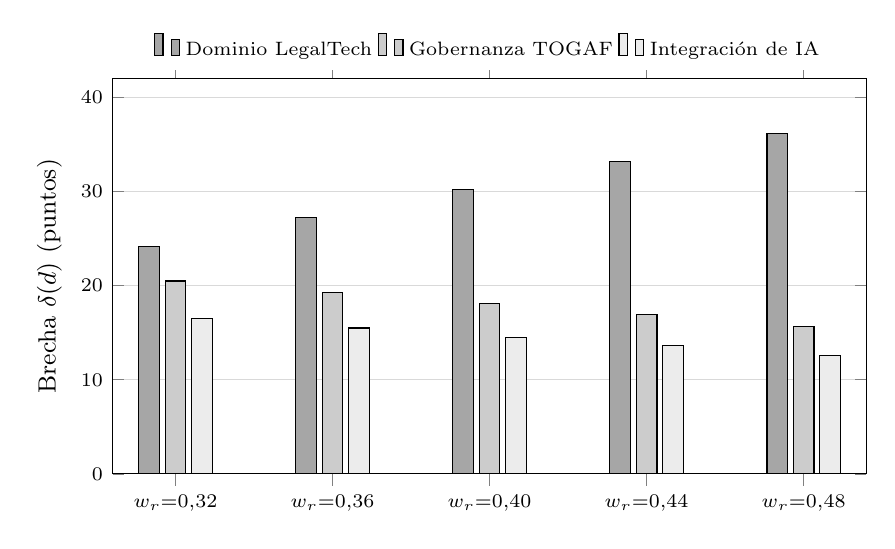
\begin{tikzpicture}
\begin{axis}[
  ybar,
  width=0.92\textwidth, height=6.6cm,
  bar width=7.5pt,
  ymin=0, ymax=42,
  ylabel={Brecha $\delta(d)$ (puntos)},
  ylabel style={font=\small},
  symbolic x coords={{$w_r{=}0{,}32$},{$w_r{=}0{,}36$},{$w_r{=}0{,}40$},{$w_r{=}0{,}44$},{$w_r{=}0{,}48$}},
  xtick=data,
  x tick label style={font=\scriptsize},
  yticklabel style={font=\scriptsize},
  legend style={font=\scriptsize, at={(0.5,1.02)}, anchor=south, legend columns=3, draw=none},
  ymajorgrids, major grid style={gray!30},
]
\addplot+[draw=black, fill=gray!70] coordinates
  {({$w_r{=}0{,}32$},24.2) ({$w_r{=}0{,}36$},27.2) ({$w_r{=}0{,}40$},30.2) ({$w_r{=}0{,}44$},33.2) ({$w_r{=}0{,}48$},36.2)};
\addplot+[draw=black, fill=gray!40] coordinates
  {({$w_r{=}0{,}32$},20.5) ({$w_r{=}0{,}36$},19.3) ({$w_r{=}0{,}40$},18.1) ({$w_r{=}0{,}44$},16.9) ({$w_r{=}0{,}48$},15.7)};
\addplot+[draw=black, fill=gray!15] coordinates
  {({$w_r{=}0{,}32$},16.5) ({$w_r{=}0{,}36$},15.5) ({$w_r{=}0{,}40$},14.5) ({$w_r{=}0{,}44$},13.6) ({$w_r{=}0{,}48$},12.6)};
\legend{Dominio LegalTech, Gobernanza TOGAF, Integración de IA}
\end{axis}
\end{tikzpicture}
\caption{Episodio E4: las tres brechas principales bajo perturbación de $\pm 20\%$ del peso raíz $w_r$ (valor nominal 0{,}40). El ordenamiento LegalTech $>$ TOGAF $>$ IA es invariante y $\Psi_{\mathrm{global}}$ varía menos de 0{,}002, evidenciando robustez de la agenda de remediación frente al juicio experto.}
\label{fig:sens}
\end{figure}

Tres lecturas sintetizan la evaluación. Primera, la \emph{complementariedad} de episodios: la verificación formal (E1) acota los defectos del modelo, el escenario artificial (E2) ejercita el motor de validación en condiciones controladas, y el despliegue naturalista (E3) demuestra utilidad sobre el fenómeno real ---el hallazgo de que solo el 36{,}7\% de los términos procesales se cumple, con el procedimiento sumario rindiendo peor (35{,}6\%) que el monitorio (40{,}0\%), es conocimiento accionable que ningún episodio artificial habría producido. Segunda, la \emph{robustez} (E4): la estabilidad del ordenamiento de brechas bajo perturbación de pesos desactiva la crítica habitual a las métricas dependientes de juicio experto. Tercera, la \emph{reflexividad} (E5): al incorporar los instrumentos de validez como endpoints del propio artefacto, la evaluación deja de ser un acto externo y se vuelve capacidad permanente de la plataforma, auditable en la bitácora encadenada.

%% ============================================================
\section{Discusión: Contribución al Conocimiento}
\label{sec:discusion}

\subsection{Posicionamiento y Principios de Diseño}
En el marco de Gregor y Hevner \cite{Gregor2013}, MALTG es una contribución de tipo \emph{mejora}: soluciones nuevas (integración de sombras semánticas, razonamiento normativo acotado, notarización y adaptación) para un problema conocido (gobernanza digital judicial no auditable). El nivel de abstracción alcanzado es el de una \emph{teoría de diseño naciente} (nivel 2): del artefacto se destilan seis principios transferibles (Tabla~\ref{tab:dp}) que otros equipos pueden reutilizar en dominios normativos de alto riesgo (salud, tributación, contratación pública), y la Tabla~\ref{tab:teoria} estructura la teoría con los ocho componentes de Gregor y Jones \cite{GregorJones2007}, respondiendo al llamado de equilibrio entre artefacto y teoría \cite{Baskerville2018}.

\begin{table}[H]
\caption{Principios de diseño destilados de la experimentación con MALTG.}
\label{tab:dp}
\begin{tabularx}{\textwidth}{lX}
\toprule
\textbf{Principio} & \textbf{Enunciado}\\
\midrule
DP1 Frontera ontológica & Para dominios donde el error genera daño jurídico, restrinja las salidas de IA al vocabulario cerrado de una ontología ejecutable; reporte lo ajeno como \emph{fuera de frontera} en lugar de generarlo.\\
DP2 Sombra antes que gemelo & Cuando la actuación sobre el sistema observado es competencia exclusiva de un tercero (la administración pública), diseñe sombras digitales de flujo unidireccional, no gemelos con retroalimentación automática \cite{Kritzinger2018}.\\
DP3 Medición del anclaje & Toda correspondencia modelo--realidad debe ser medible: defina funciones de cobertura y brecha ($\Psi$, $\delta$) computables en cada ciclo de ingesta \cite{Karabulut2024}.\\
DP4 Procedencia total & Cada salida debe portar su derivación (regla, artículo, fechas, hash de la base normativa) para ser re-derivable por terceros.\\
DP5 Integridad encadenada & Notarice tanto el objeto de estudio (expediente) como la operación del propio artefacto (bitácora) con cadenas de hashes \cite{Haber1991}.\\
DP6 Rigor instrumentado & Incorpore los instrumentos de validez (gold standard, AHP, CVR, sensibilidad, concordancia) como componentes operativos del artefacto, no como análisis externos irrepetibles.\\
\bottomrule
\end{tabularx}
\end{table}

\begin{table}[H]
\caption{MALTG como teoría de diseño naciente según los ocho componentes de Gregor y Jones \cite{GregorJones2007}.}
\label{tab:teoria}
\begin{tabularx}{\textwidth}{lX}
\toprule
\textbf{Componente} & \textbf{Instanciación en MALTG}\\
\midrule
Propósito y alcance & Gobernanza automatizada, fundada, verificable y adaptativa de ecosistemas digitales en dominios normativos de alto riesgo.\\
Constructos & $\Psi$, $\delta$, $S$, IVF, IDP, $\rho$, $\mathcal{H}$, niveles de madurez (Tabla~\ref{tab:tipos}).\\
Principios de forma y función & DP1--DP6 (Tabla~\ref{tab:dp}); arquitectura de capas de la Figura~\ref{fig:arch}.\\
Mutabilidad del artefacto & Ciclo MAPE-K: changelog normativo, recalibración empírica, supuestos acotados min--max con asiento en bitácora.\\
Proposiciones comprobables & (i) $\mathcal{H}=0$ sobre el dominio tipificado; (ii) evidencia de manipulación de la cadena; (iii) estabilidad del ordenamiento de brechas bajo perturbación de pesos.\\
Conocimiento justificativo & Gemelos/sombras \cite{Jones2020,Brauner2022}; ingeniería ontológica \cite{Gruber1993,Guarino2002}; conformidad \cite{Rozinat2008}; criptografía \cite{Haber1991}; autonomía \cite{Kephart2003}.\\
Principios de implementación & Contenedorización; API REST; datos abiertos JSON-LD/DCAT \cite{Guha2016}; separación estricta razonador/generador.\\
Instanciación expositiva & Plataforma MALTG evaluada en el ecosistema de justicia del Ecuador (Secciones~\ref{sec:escenario} y \ref{sec:eval}).\\
\bottomrule
\end{tabularx}
\end{table}

\subsection{Limitaciones}
Primero, el episodio E5 está instrumentado pero la anotación del estándar de oro por panel de juristas independientes está en curso; hasta su cierre, $F_1$ y $\kappa$ del reconocimiento de actos deben tratarse como protocolo y no como resultado. Segundo, la evaluación naturalista cubre una institución y dos procedimientos dominantes; la generalización empírica exige replicación multi-institucional, aunque la generalización \emph{teórica} ---los principios DP1--DP6--- descansa en mecanismos independientes del caso \cite{Gregor2013}. Tercero, las puntuaciones ontológicas y los pesos incorporan juicio experto; los instrumentos A3 (AHP con CR, sensibilidad) y Delphi (concordancia $r_s$) lo disciplinan pero no lo eliminan. Cuarto, la sombra observa la superficie pública del ecosistema: sus índices son cotas inferiores de la madurez real. Quinto, la cadena de hashes es centralizada con raíz publicable; su anclaje en una DLT interinstitucional \cite{Olnes2017} es extensión natural que no altera el modelo formal.

%% ============================================================
\section{Conclusiones}
\label{sec:conclusions}

Este artículo aplicó ciencia del diseño de extremo a extremo ---tres ciclos \cite{Hevner2004}, seis actividades DSRM \cite{Peffers2007}, evaluación FEDS multi-episodio \cite{Venable2016} y destilación teórica \cite{Gregor2013,GregorJones2007}--- para construir MALTG, una suite integrada de artefactos de gobernanza digital judicial evaluada en el ecosistema de justicia del Ecuador. La experimentación produjo resultados verificables en tres planos: el \emph{técnico} (cobertura $\Psi_{\mathrm{global}} = 0{,}905$ con robustez demostrada; $\mathcal{H} = 0$ por construcción; integridad encadenada), el \emph{empírico} (madurez institucional 46/100; puntualidad procesal 36{,}7\% sobre 60 términos de 47 causas reales; agenda de brechas estable) y el \emph{teórico} (seis principios de diseño y una teoría naciente para artefactos de gobernanza en dominios normativos de alto riesgo). El trabajo futuro prioriza el cierre del episodio E5 con panel de juristas independientes, la replicación multi-institucional para transitar de teoría naciente a teoría de diseño madura, y el anclaje interinstitucional de la notarización.

\vspace{6pt}

\authorcontributions{Conceptualización, metodología, software, validación, redacción: P.M.A. El autor ha leído y aceptado la versión publicada del manuscrito.}

\funding{Esta investigación no recibió financiación externa.}

\institutionalreview{No aplicable. Los expedientes procesados son registros públicos del sistema oficial de consulta de procesos judiciales del Ecuador.}

\informedconsent{No aplicable.}

\dataavailability{El código fuente de la plataforma MALTG, las ontologías OWL, las sombras digitales JSON-LD, la base de conocimiento COGEP y los datos de evaluación están disponibles a solicitud al autor de correspondencia.}

\conflictsofinterest{El autor declara no tener conflictos de interés. Los indicadores generados por el sistema son instrumentos de apoyo a la gestión y no constituyen asesoría jurídica.}

%% ============================================================
\begin{adjustwidth}{-\extralength}{0cm}
\reftitle{Referencias}
\bibliography{references}
\end{adjustwidth}

\end{document}
